\heading{数学物理方法（上）-第13次作业}

\begin{question}
计算下列积分：

\begin{enumerate}
  \item \(\displaystyle\int_0^\infty \frac{x^{\alpha - 1} \ln x}{1-x^2}\dd{x},\ 0<\alpha<2\);

  \item \(\displaystyle\int_0^\infty \frac{\ln^2 x}{(x+a)(x+b)}\dd{x},\ b>a>0\);

  \item \(\displaystyle\operatorname{v.p.}\int_0^\infty \frac{dx}{1+x-x^2}\).
\end{enumerate}
\begin{solution}
\begin{enumerate}
  \item
\textbf{留数定理法}\par

先计算参数积分
\[
J(\alpha)=\operatorname{v.p.}\int_0^\infty
\frac{x^{\alpha-1}}{1-x^2}\dd{x},
\qquad 0<\alpha<2.
\]
取
\[
g(z)=\frac{z^{\alpha-1}}{1-z^2},
\qquad 0<\arg z<2\pi,
\]
并使用绕正实轴的钥匙孔围道，在 \(z=1\) 处作对称小圆弧绕行。
围道示意如下。
\begin{center}
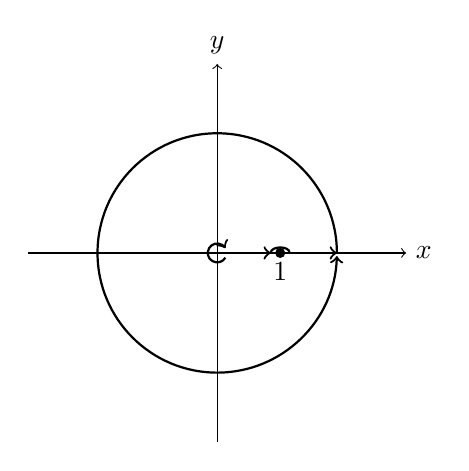
\begin{tikzpicture}[scale=0.8]
  \draw[->] (-3,0) -- (3,0) node[right] {$x$};
  \draw[->] (0,-3) -- (0,3) node[above] {$y$};
  % Keyhole: small circle around origin, large arc, with indentation at z=1
  \draw[thick,->] (-30:0.15) arc (-30:-330:0.15);
  \draw[thick,->] (0.15,0) -- (0.85,0);
  \draw[thick] (0.85,0) to[out=90,in=90] (1.15,0);
  \draw[thick,->] (1.15,0) -- (1.9,0);
  \draw[thick,->] (1.9,0) arc (0:358.5:1.9);
  \filldraw (1,0) circle (2pt);
  \node at (1,0) [below] {$1$};
\end{tikzpicture}
\end{center}
由上下岸积分、\(z=-1\) 处的留数以及 \(z=1\) 两侧小圆弧的贡献，
可得
\[
J(\alpha)=\frac{\pi}{2}\cot\frac{\pi\alpha}{2}.
\]
在 \(0<\alpha<2\) 内对参数求导，便有
\[
\begin{aligned}
\int_0^\infty\frac{x^{\alpha-1}\ln x}{1-x^2}\dd{x}
&=J'(\alpha)\\
&=-\frac{\pi^2}{4}\csc^2\frac{\pi\alpha}{2}.
\end{aligned}
\]

\textbf{费曼积分法}\par

考察 \(f(z) = \dfrac{z^{\alpha-1}}{1-z^2}\)，有 \[ \int_0^\infty \frac{x^{\alpha-1}}{1-x^2}\dd{x}\overset{t=x^2}{=} \frac12\int_0^\infty \frac{t^{\alpha/2-1}}{1-t}\dd{t}=\frac12 \int_0^1 \frac{t^{\alpha/2-1}}{1-t}\dd{t}+\frac12 \int_1^\infty \frac{t^{\alpha/2-1}}{1-t}\dd{t} \] \[ =\frac12 \int_0^1 \frac{t^{\alpha/2-1}-t^{-\alpha/2}}{1-t}\dd{t} \]

注意到有，\(\psi(x)=-\gamma +\displaystyle\int_0^1 \frac{1-t^{x-1}}{1-t}\dd{t}\)，则有 \[ \int_0^1 \frac{t^{p-1}-t^{q-1}}{1-t}\dd{t}=\psi(q)-\psi(p) \]
因此有，\[ \int_0^\infty \frac{x^{\alpha-1}}{1-x^2}\dd{x}=\frac12\bigl(\psi(-\alpha/2+1)-\psi(\alpha/2)\bigr)=\frac{\pi}{2}\cot\frac{\pi\alpha}{2} \]

最后可以得到，\[ \int_0^\infty \frac{x^{\alpha-1} \ln x}{1-x^2}\dd{x} = \pdv{}{\alpha} \biggl(\int_0^\infty \frac{x^{\alpha-1}}{1-x^2}\dd{x}\biggr)=-\frac{\pi^2}{4\sin^2(\pi\alpha/2)} \]

  \item
\textbf{留数定理法}\par

我们设 \(f_j (x)= \dfrac{(\ln x)^j}{(x+a)(x+b)}\)，不妨先计算一些必要的表达式：\[ \operatorname{res}\{f_j (x),-a\}=\frac{1}{b-a} (\ln a+\pi\ii)^j,\quad \operatorname{res}\{f_j (x),-b\}=\frac{1}{a-b} (\ln b + \pi\ii)^j \]

因此考察玦形围道可以得到 \[ \oint_C f_j (z)\dd{z} = \int_\delta^R \frac{(\ln x)^j}{(x+a)(x+b)}\dd{x}+ \int_{C_R} f_j (z)\dd{z} \] \[ +\int_R^\delta \frac{(\ln x + 2\pi\ii)^j}{(x+a)(x+b)}\dd{x}+\int_{C_\delta} f_j (z)\dd{z} \] \[ =\frac{2\pi\ii}{b-a} \bigl[(\ln a + \pi\ii)^j-(\ln b + \pi\ii)^j\bigr] \]
值得注意的是，\(\displaystyle\lim_{z\to0} z f_j (z)=0,\quad \lim_{z\to\infty} z f_j (z)=0\)
因此可以得到，\[ \int_0^\infty \frac{(\ln x)^j-(\ln x+2\pi\ii)^j}{(x+a)(x+b)}\dd{x}= \frac{2\pi\ii}{b-a}\bigl[(\ln a+\pi\ii)^j - (\ln b + \pi\ii)^j\bigr] \]
设 \(I_j=\displaystyle\int_0^\infty f_j (x)\dd{x}\)，则有 \[ \sum_{n=1}^j \binom{j}{n} I_{j-n} (2\pi\ii)^n = \frac{2\pi\ii}{b-a}\bigl[(\ln b + \pi\ii)^j - (\ln a + \pi\ii)^j\bigr] \]
故可以得到递推关系式：
\[ I_{j-1} = \frac1j \sum_{n=2}^j \binom{j}{n} I_{j-n} (2\pi\ii)^{n-1} + \frac1{j(b-a)}\bigl[(\ln b+\pi\ii)^j - (\ln a+\pi\ii)^j\bigr] \]
因此有，\[ I_0 = \frac{1}{b-a} \ln\frac{b}{a} \] \[ I_1 =\frac{1}{2(b-a)}\bigl[(\ln b + \pi\ii)^2-(\ln a+\pi\ii)^2\bigr] -\frac12\binom{2}{2}I_0\cdot (2\pi\ii) \] \[ I_2 = \frac{1}{3(b-a)} \bigl[(\ln b + \pi\ii)^3-(\ln a + \pi\ii)^3\bigr] - \frac13 \bigl(\binom{3}{2} I_1\cdot (2\pi\ii) + \binom{3}{3} I_0\cdot (2\pi\ii)^2\bigr) \]

代入计算可以得到，
\[ I_2=\frac{1}{3(b-a)} \ln\frac{b}{a} \bigl[(\ln a)^2+\ln a\ln b + (\ln b)^2 +\pi^2\bigr]=\frac{\pi^2 \ln\frac{b}{a}-(\ln a)^3+(\ln b)^3}{3(b-a)} \]

\textbf{费曼积分法}\par

考察 \(f(x)= \dfrac{x^m}{(x+a)(x+b)}\ (m<1)\)，有考察玦形围道，则 \[ \oint_C f(z)\dd{z}=\int_\delta^R \frac{x^m}{(x+a)(x+b)}\dd{x}+\int_{C_R} f(z)\dd{z} + \int_R^\delta \frac{x^m}{(x+a)(x+b)} \ee^{2\pi m\ii}\dd{x}+\int_{C_\delta} f(z)\dd{z} \] \[ =2\pi\ii \frac{(-a)^m-(-b)^m}{b-a} = 2\pi\ii \frac{a^m - b^m}{b-a} \ee^{\pi m\ii} \]

有 \(\displaystyle\lim_{z\to\infty} z f(z)=0,\ \lim_{z\to0} z f(z)=0\)，因此有 \[ \int_0^\infty \frac{x^m}{(x+a)(x+b)}\dd{x}=\frac{\pi}{\sin\pi m} \frac{a^m-b^m}{a-b} \]
最后可以得到 \[ \pdv{^2}{m^2}\int_0^\infty \frac{x^m}{(x+a)(x+b)}\dd{x}=\int_0^\infty \frac{(\ln x)^2 x^m}{(x+a)(x+b)}\dd{x} \] \[ =\frac{\pi\csc(m\pi)}{a-b} \biggl[(a^m - b^m) \pi^2 (\cot^2(m\pi) + \csc^2(m\pi)) \] \[ + a^m (\ln a)^2 - b^m (\ln b)^2 - 2\pi\cot(m\pi) (a^m \ln a - b^m \ln b)\biggr] \]
取 \(m\to0\)，有 \[ \int_0^\infty \frac{(\ln x)^2}{(x+a)(x+b)}\dd{x}=\frac{\pi^2 \ln\frac{b}{a}-(\ln a)^3+(\ln b)^3}{3(b-a)} \]

  \item
\textbf{留数定理法}\par

考察函数 \(f(z) = \dfrac{\ln z}{1+z-z^2}\)，令 \(\varphi=\dfrac{\sqrt5+1}{2}\)，考察玦形围道，有
\begin{center}
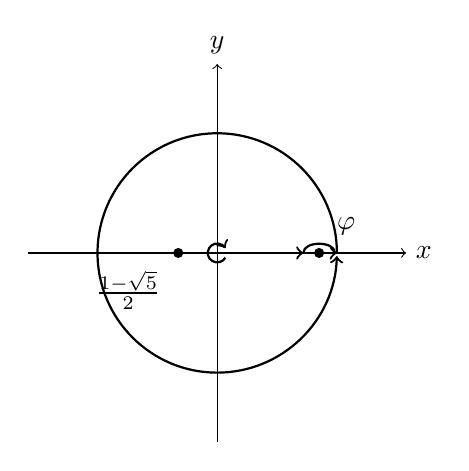
\begin{tikzpicture}[scale=0.8]
  \pgfmathsetmacro{\phi}{(sqrt(5)+1)/2}
  \pgfmathsetmacro{\psip}{(1-sqrt(5))/2}
  \draw[->] (-3,0) -- (3,0) node[right] {$x$};
  \draw[->] (0,-3) -- (0,3) node[above] {$y$};
  % Keyhole
  \draw[thick,->] (-30:0.15) arc (-30:-330:0.15);
  \draw[thick,->] (0.15,0) -- ({\phi-0.25},0);
  \draw[thick] ({\phi-0.25},0) to[out=90,in=90] ({\phi+0.25},0);
  \draw[thick,->] ({\phi+0.25},0) -- (1.9,0);
  \draw[thick,->] (1.9,0) arc (0:358.5:1.9);
  % Golden ratio point
  \filldraw ({\phi},0) circle (2pt);
  \node at ({\phi},0) [above right=3pt] {$\varphi$};
  % Negative root
  \filldraw ({\psip},0) circle (2pt);
  \node at ({\psip},0) [below left=3pt] {$\frac{1-\sqrt5}{2}$};
\end{tikzpicture}
\end{center}

\[ \oint_C f(z)\dd{z} =\biggl(\int_{\delta_1}^{\varphi-\delta_2}+\int_{\varphi+\delta_2}^{R}\biggr) \frac{\ln x}{1+x-x^2}\dd{x} + \int_{C_R} f(z)\dd{z} \] \[ +\biggl(\int_{\varphi-\delta_2}^{\delta_1}+\int_{R}^{\varphi+\delta_2}\biggr) \frac{\ln x + 2\pi\ii}{1+x-x^2}\dd{x} +\int_{C_{\delta_1}} f(z)\dd{z} + \int_{C_{\delta_2}} f(z)\dd{z} \] \[ = 2\pi\ii \operatorname{res}\biggl\{f(z),\frac{1-\sqrt5}{2}\biggr\}= \frac{2\pi\ii}{\sqrt5} \bigl(\ln (1/\varphi)+\pi\ii\bigr) \]
根据大圆弧引理，有 \(\displaystyle\lim_{z\to\infty} \frac{z\ln z}{1+z-z^2}=0\)，因此 \(\displaystyle \lim_{z\to\infty} \int_{C_R} f(z)\dd{z}= 0\)
根据小圆弧引理，有 \[ \lim_{z\to0} \frac{z\ln z}{1+z-z^2}=0,\ \lim_{z\to\varphi} \frac{(z-\varphi)\ln z}{1+z-z^2}=-\frac1{\sqrt5}\ln\varphi,\ \lim_{z\to\varphi \ee^{2\pi\ii}} \frac{(z-\varphi)\ln z}{1+z-z^2}=-\frac{1}{\sqrt5}(\ln\varphi+2\pi\ii) \]
因此
\[
\lim_{\delta_1\to0}\int_{C_{\delta_1}}f(z)\dd{z}=0,
\qquad
\lim_{\delta_2\to0}\int_{C_{\delta_2}}f(z)\dd{z}
=\frac{2\pi\ii}{\sqrt5}\bigl(\ln\varphi+\pi\ii\bigr).
\]
综上有
\[
-2\pi\ii\operatorname{v.p.}\int_0^\infty\frac{\dd{x}}{1+x-x^2}
=-\frac{2\pi\ii}{\sqrt5}
\left(\ln\varphi-\ln\frac1\varphi\right),
\]
因此
\[
\operatorname{v.p.}\int_0^\infty\frac{\dd{x}}{1+x-x^2}
=\frac{2}{\sqrt5}\ln\varphi.
\]

\textbf{定积分法}\par

部分分式分解给出
\[
\int\frac{\dd{x}}{1+x-x^2}
=-\frac1{\sqrt5}\ln\frac{x-\varphi}{x+1/\varphi}.
\]

在 \(x=\varphi\) 两侧对称取极限，得到
\[
\begin{aligned}
\operatorname{v.p.}\int_0^\infty\frac{\dd{x}}{1+x-x^2}
&=\frac{2}{\sqrt5}\ln\varphi
-\frac1{\sqrt5}\lim_{\delta\to0}
\ln\frac{\sqrt5-\delta}{\sqrt5+\delta}\\
&=\frac{2}{\sqrt5}\ln\varphi.
\end{aligned}
\]
\end{enumerate}
\end{solution}
\end{question}

\begin{question}
任意一个二阶线性常微分方程都可以写成

\[ \dv[2]{y}{x}+a(x)\dv{y}{x}+b(x)y(x)=c(x) \]
其中 \(a(x),b(x),c(x)\) 都是已知函数，请将方程化为如下形式：
\[ \dv{}{x}\bigl[p(x)\dv{y}{x}\bigr] + q(x)y(x)=f(x) \]
即请将 \(p(x),q(x),f(x)\) 用 \(a(x),b(x),c(x)\) 表示。
\begin{solution}
通过一些计算，可以得到
\[ \dv{}{x}\bigl[p(x)\dv{y}{x}\bigr] + q(x)y(x)=f(x) \] \[ p(x)\dv[2]{y}{x}+\dv{p}{x}\dv{y}{x}+q(x)y(x)=f(x) \] \[ \dv[2]{y}{x}+\frac{p'(x)}{p(x)}\dv{y}{x}+\frac{q(x)}{p(x)}y(x)=\frac{f(x)}{p(x)} \]
对比系数可以得到 \[ \frac{p'(x)}{p(x)}=a(x)\ \Rightarrow\ p(x)=p(x_0)\exp\biggl(\int_{x_0}^x a(x)\dd{x}\biggr) \] \[ q(x)=b(x)p(x)=b(x)p(x_0)\exp\biggl(\int_{x_0}^x a(x)\dd{x}\biggr) \] \[ f(x)=c(x)p(x)=c(x)p(x_0)\exp\biggl(\int_{x_0}^x a(x)\dd{x}\biggr) \]
\end{solution}
\end{question}

\begin{question}
分析扩充的复平面 \(\overline{\mathbb{C}}\) 中下列方程的奇点，并且指出其是否为正则奇点。
\begin{enumerate}
  \item \(z u''+(b-z) u'-a u =0\)，其中 \(a,b\) 为已知常数；
  \item \((1-z^2) v''-2(m+1)z v'+(\lambda-m(m+1)) v= 0\)，其中 \(\lambda,m\) 为已知常数。
\end{enumerate}
\begin{solution}
\begin{enumerate}
  \item 在 \(\mathbb{C}\) 上，奇点为 \(z=0\)，且为正则奇点。对于 \(\infty\)，作变换 \(t=1/z\)，则
  \[
  t^3\dv[2]{u}{t}
  +\bigl[(2-b)t^2+t\bigr]\dv{u}{t}
  -au=0.
  \]
  除以 \(t^3\) 得
  \[
  \dv[2]{u}{t}
  +\left(\frac{2-b}{t}+\frac1{t^2}\right)\dv{u}{t}
  -\frac{a}{t^3}u=0.
  \]
  一阶导数项系数在 \(t=0\) 有二阶极点，所以 \(t=0\) 不是正则奇点，即 \(z=\infty\) 为非正则奇点。
  \item 在 \(\mathbb{C}\) 上，奇点为 \(z=\pm1\) 处，显然均为正则奇点。对于 \(\infty\)，作变换 \(t=1/z\)，\(\displaystyle\dv{}{z}=-t^2\dv{}{t}\)，因此有 \[ (t^2-1)\dv{}{t}\bigl[t^2\dv{v}{t}\bigr]+2(m+1)t\dv{v}{t}+(\lambda-m(m+1))v \] \[ =(t^2-1)t^2\dv[2]{v}{t}+2t(m+t^2)\dv{v}{t}+(\lambda-m(m+1))v=0 \]因此有，\[ \dv[2]{v}{t}+\frac{2(m+t^2)}{(t^2-1)t}\dv{v}{t}+\frac{\lambda-m(m+1)}{t^2(t^2-1)}v=0 \]可见 \(t=0\) 为 \(\frac{2(m+t^2)}{t(t^2-1)}\) 的一阶极点，为 \(\frac{\lambda-m(m+1)}{t^2(t^2-1)}\) 的二阶极点，故可见 \(t=0\) 为方程的正则奇点，即 \(z=\infty\) 为方程的正则奇点。
\end{enumerate}
\end{solution}
\end{question}

\begin{question}
计算在 \(\overline{\mathbb{C}}\) 上下列微分方程在正则奇点处的指标：
\begin{enumerate}
  \item \(z(1-z)\dfrac{d^2u}{dz^2}+[\gamma-(\alpha+\beta+1)z]\dfrac{du}{dz}-\alpha\beta u=0\)；
  \item \(u''-2z u'+2\lambda u=0\)；
  \item \((1-z^2)v''-2(m+1)z v'+(\lambda-m(m+1))v=0\)；
  \item \((1-z^2)\dfrac{d^2w}{dz^2}-2z\dfrac{dw}{dz}+\nu(\nu+1)w=0\)。
\end{enumerate}
\begin{solution}
\begin{enumerate}
  \item 有该微分方程的标准形式为 \[ \dv[2]{u}{z}+\frac{\gamma-(\alpha+\beta+1)z}{z(1-z)}\dv{u}{z}-\frac{\alpha\beta}{z(1-z)}u=0 \]容易看到，微分方程的正则奇点为 \(z=0,1\)。\ 在 \(z=0\) 处，有指标方程 \(\rho(\rho-1)+\gamma\rho-0=0\)可以解得 \(\rho=0\) 或 \(1-\gamma\)。\ 在 \(z=1\) 处，有指标方程 \(\rho(\rho-1)+(\alpha+\beta-\gamma+1)\rho+0=0\)可以解得 \(\rho=0\) 或 \(\gamma-\alpha-\beta\)。\ 作变换 \(t=1/z\)，\(\displaystyle\dv{}{z}=-t^2\dv{}{t}\)，可以得到 \[ (t-1)\dv{}{t}\bigl[t^2\dv{u}{t}\bigr]-t^2\bigl[\gamma-(\alpha+\beta+1)/t\bigr]\dv{u}{t}-\alpha\beta u=0 \]因此可以得到，\[ \dv[2]{u}{t}+\frac{\alpha+\beta-1+(2-\gamma)t}{t(t-1)}\dv{u}{t}-\frac{\alpha\beta}{t^2(t-1)}u=0 \]容易看到，微分方程的正则奇点为 \(t=0\)，即 \(z=\infty\)，故有指标方程 \(\rho(\rho-1)-(\alpha+\beta-1)\rho+\alpha\beta=0\)可以解得 \(\rho=\alpha\) 或 \(\beta\)。

  \item 作变换 \(t=1/z\)，\(\displaystyle\dv{}{z}=-t^2\dv{}{t}\)，可以得到 \[ t^2\dv{}{t}\bigl[t^2\dv{u}{t}\bigr]+2t\dv{u}{t}+2\lambda u=0 \]因此有 \[ \dv[2]{u}{t}+\frac{2t^2+2}{t^3}\dv{u}{t}+\frac{2\lambda}{t^4}u=0 \]由此可见 \(t=0\) 处不是 \(u\) 的正则奇点。方程在 \(\overline{\mathbb{C}}\) 上没有正则奇点。

  \item 有该微分方程的标准形式为，\[ \dv[2]{v}{z}+\frac{2(m+1)z}{z^2-1}\dv{v}{z}+\frac{\lambda-m(m+1)}{1-z^2}v=0 \]容易看到，微分方程的正则奇点为 \(z=\pm1\)。\ 在 \(z=1\) 处，有指标方程，\(\rho(\rho-1)+(m+1)\rho+0=0\)可以解得 \(\rho=0\) 或 \(-m\)。\ 在 \(z=-1\) 处，有指标方程，\(\rho(\rho-1)+(m+1)\rho+0=0\)可以解得 \(\rho=0\) 或 \(-m\)。\ 作变换 \(t=1/z\)，\(\displaystyle\dv{}{z}=-t^2\dv{}{t}\)，可以得到 \[ \dv[2]{v}{t}+\frac{2(m+t^2)}{(t^2-1)t}\dv{v}{t}+\frac{\lambda-m(m+1)}{t^2(t^2-1)}v=0 \]容易看到，微分方程的正则奇点为 \(t=0\)，即 \(z=\infty\)，故有指标方程 \(\rho(\rho-1)-2m\rho-[\lambda-m(m+1)]=0\)解得 \(\rho_{1,2}=\dfrac{2m+1\pm\sqrt{4\lambda+1}}{2}\)

  \item 标准形式为
  \[
  \dv[2]{w}{z}-\frac{2z}{1-z^2}\dv{w}{z}
  +\frac{\nu(\nu+1)}{1-z^2}w=0.
  \]
  \(z=\pm1\) 均为正则奇点，两处的指标均为 \(0,0\)。作变换
  \(t=1/z\) 后得到
  \[
  \dv[2]{w}{t}
  +\frac{2t}{t^2-1}\dv{w}{t}
  +\frac{\nu(\nu+1)}{t^2(t^2-1)}w=0.
  \]
  因此 \(t=0\)，即 \(z=\infty\)，也是正则奇点。此时指标方程为
  \[
  \rho(\rho-1)-\nu(\nu+1)=0,
  \]
  故指标为 \(\rho=\nu+1\) 或 \(\rho=-\nu\)。
\end{enumerate}
\end{solution}
\end{question}

\begin{question}
求下列方程在 \(z=0\) 邻域内的两个线性无关级数解：
\begin{enumerate}
  \item \((1+z+z^2) w''(z)+2(1+2z) w'(z)+2 w(z)=0\)
  \item \(z w''(z)-z w'(z)+w(z)=0\)
\end{enumerate}
\begin{solution}
\begin{enumerate}
  \item 在 \(z=0\) 处的指标方程为 \(\rho(\rho-1)=0\)可以解得 \(\rho_{1,2}=1,0\)。将 \(w_1=z^{\rho_1}\sum_{n=0}^\infty c_n z^n\) 代入微分方程，可以得到 \[ (1+z+z^2)\sum_{n=0}^\infty (\rho+n)(\rho+n-1)c_n z^{\rho+n-2}+2(1+2z)\sum_{n=0}^\infty (\rho+n)c_n z^{\rho+n-1}+2\sum_{n=0}^\infty c_n z^{\rho+n}=0 \] \[ \sum_{n=0}^\infty (\rho+n)(\rho+n-1)c_n z^{\rho+n-2}+\sum_{n=0}^\infty (\rho+n)(\rho+n+1)c_n z^{\rho+n-1}+\sum_{n=0}^\infty (\rho+n+1)(\rho+n+2)c_n z^{\rho+n}=0 \]对于 \(z^{\rho-2}\) 项，有 \(c_0\rho(\rho-1)=0\)。对于 \(z^{\rho-1}\) 项，有 \(c_1(\rho+1)\rho+c_0\rho(\rho+1)=0\)。对于 \(z^{\rho-2+n}\ (n\ge 2)\) 项，有 \[ c_n (\rho+n)(\rho+n-1)+c_{n-1}(\rho+n-1)(\rho+n)+c_{n-2}(\rho+n-1)(\rho+n)=0 \]综上可以得到递推关系式：\(c_1+c_0=0,\quad c_n+c_{n-1}+c_{n-2}=0\)简单计算可以得到 \[ c_n=\begin{cases} c_0 & n\equiv0\pmod3,\\ -c_0 & n\equiv1\pmod3,\\ 0 & n\equiv2\pmod3 \end{cases} \]即可以得到 \[ w_1(z)=z\sum_{n=0}^\infty c_0(z^{3n}-z^{3n+1}) \]利用Frobenius方法的结论，可以得到方程的另一个级数解。令 \(c_0=c'_0(\rho-\rho_2)\)，有 \[ w_2(z)=\ln z\cdot z^{\rho}\sum_{n=0}^\infty \bigl.c_n\bigr|_{\rho=\rho_2} z^n+z^{\rho}\sum_{n=0}^\infty \bigl.\dv{c_n}{\rho}\bigr|_{\rho=\rho_2}z^n =\sum_{n=0}^\infty c'_0(z^{3n}-z^{3n+1}) \]综上所述，有 \[ w_1(z)=\sum_{n=0}^\infty c_0(z^{3n+1}-z^{3n+2}),\quad w_2(z)=\sum_{n=0}^\infty c'_0(z^{3n}-z^{3n+1}) \]

  \item 在 \(z=0\) 处的指标方程为 \(\rho(\rho-1)=0\)，可以解得 \(\rho_{1,2}=1,0\)。将 \(w_1(z)=z^{\rho}\sum_{n=0}^\infty c_n z^n\) 代入微分方程，可以得到 \[ z\sum_{n=0}^\infty (\rho+n)(\rho+n-1)c_n z^{\rho+n-2}-z\sum_{n=0}^\infty (\rho+n)c_n z^{\rho+n-1}+\sum_{n=0}^\infty c_n z^{\rho+n}=0 \] \[ \sum_{n=0}^\infty (\rho+n)(\rho+n-1)c_n z^{\rho+n-1}-\sum_{n=0}^\infty (\rho+n-1)c_n z^{\rho+n}=0 \] \[ \rho(\rho-1)c_0 z^{\rho-1}+\sum_{n=1}^\infty \bigl[(\rho+n)(\rho+n-1)c_n-(\rho+n-2)c_{n-1}\bigr]z^{\rho+n-1}=0 \]这要求，\[ c_n = c_{n-1}\frac{\rho+n-2}{(\rho+n)(\rho+n-1)} = c_{n-1}\cdot\frac{\Gamma(\rho+n-1)/\Gamma(\rho+n-2)}{\Gamma(\rho+n+1)/\Gamma(\rho+n)\cdot\Gamma(\rho+n)/\Gamma(\rho+n-1)} \] \[ c_n\cdot\frac{\Gamma(\rho+n+1)\Gamma(\rho+n)}{\Gamma(\rho+n-1)} =c_{n-1}\cdot\frac{\Gamma(\rho+n)\Gamma(\rho+n-1)}{\Gamma(\rho+n-2)}=\dots =c_0\frac{\Gamma(\rho+1)\Gamma(\rho)}{\Gamma(\rho-1)} \]因此可以解得，\[ c_n = c_0\frac{(\rho-1)\Gamma(\rho+1)}{(\rho+n-1)\Gamma(\rho+n+1)} \]当 \(\rho=1\) 时，有 \(c_n=0\ (n\ge 1)\)，因此有 \(w_1(z)=c_0z\)。当 \(\rho=0\) 时，根据Frobenius方法的结论，有 \[ w_2(z)=\ln z\cdot\sum_{n=0}^\infty \bigl.c_n\bigr|_{\rho=0} z^{n}+\sum_{n=0}^\infty \bigl.\dv{c_n}{\rho}\bigr|_{\rho=0} z^{n} \]当 \(\rho=0\) 时，取 \(c_0=c'_0\rho\)，有 \(c_1=\displaystyle\lim_{\rho\to0} c_0\cdot\frac{-1\Gamma(1)}{\rho\Gamma(2)}=-c'_0\)，对于 \(n\ge 2\)，都有 \(c_n=0\)。又有 \[ \bigl.\dv{c_n}{\rho}\bigr|_{\rho=0} =\bigl.\dv{c_0}{\rho}\bigr|_{\rho=0}\cdot\frac{(\rho-1)\Gamma(\rho+1)}{(\rho+n-1)\Gamma(\rho+n+1)}+\cancel{c_0\dv{}{\rho}\Bigl[\frac{(\rho-1)\Gamma(\rho+1)}{(\rho+n-1)\Gamma(\rho+n+1)}\Bigr]}^{\displaystyle \bigl.c_0\bigr|_{\rho=0}=0} \] \[ =c'_0\frac{-1\Gamma(1)}{(n-1)\Gamma(n+1)}=\frac{-c'_0}{(n-1)n!}\quad (n\neq2) \] \[ \bigl.\dv{c_1}{\rho}\bigr|_{\rho=0} =\bigl.\dv{}{\rho}\Bigl(\frac{c'_0(\rho-1)\Gamma(\rho+1)}{\Gamma(\rho+2)}\Bigr)\bigr|_{\rho=0}=c'_0\bigl.\dv{}{\rho}\Bigl(\frac{\rho-1}{\rho+1}\Bigr)\bigr|_{\rho=0}=2c'_0 \]代入有，\[ w_2(z)=-c'_0 z\ln z+c'_0+2c'_0 z-c'_0\sum_{n=2}^\infty \frac{z^n}{(n-1)n!} \]综合上述两个结果，可以得到 \[ w_1(z)=c_0z,\quad w_2(z)=c'_0\Bigl[1+2z-z\ln z-\sum_{n=2}^\infty \frac{z^n}{(n-1)n!}\Bigr] \]
\end{enumerate}
\end{solution}
\end{question}

\begin{question}
当参数 \(\lambda\) 取何值时Laguerre方程 \(x y''+(1-x)y'+\lambda y=0\) 在 \(x=0\) 处有一解截断为多项式？并求出此多项式解。
\begin{solution}
取指标 \(\rho=0\)，令 \(y(x)=\sum_{n=0}^{\infty}c_nx^n\)。代入方程并比较系数，得到
\[
c_n=-\frac{\lambda-n+1}{n^2}c_{n-1},
\qquad n\ge1.
\]
级数在 \(n=N\) 后截断，当且仅当
\(\lambda=N\in\mathbb{Z}_{\ge0}\)。此时
\[
c_n=(-1)^n\frac{N!}{(N-n)!\,(n!)^2}c_0,
\qquad 0\le n\le N,
\]
所以多项式解为
\[
y_N(x)
=c_0\sum_{n=0}^{N}(-1)^n\binom{N}{n}\frac{x^n}{n!}
=c_0L_N(x).
\]
\end{solution}
\end{question}

\begin{question}
求 Legendre 方程
\[
\frac{d}{dz}\Bigl[(1-z^2)\frac{dw}{dz}\Bigr] + \mu(\mu+1) w(z)=0
\]
在 $z=1$ 的有界解，其中 $\mu$ 为已知复数。
\begin{solution}
有该微分方程可以化简为
\[
(1-z^2)\dv[2]{w}{z} - 2z\dv{w}{z} + \mu(\mu+1) w(z)=0.
\]
令 $y=z-1$，有
\[
-y(y+2)\dv[2]{w}{y} - 2(y+1)\dv{w}{y} + \mu(\mu+1) w(y)=0.
\]
其对应的指标方程为
\[
\rho(\rho-1) + \rho = 0,
\]
因此可以解得 $\rho_{1,2}=0$（二重根）。将 $w(y)=\sum_{n=0}^\infty c_n y^n$ 代入微分方程，可以得到
\[
\sum_{n=0}^\infty 2n^2 c_n y^{n-1} + \sum_{n=0}^\infty \bigl[n(n+1)-\mu(\mu+1)\bigr] c_n y^n =0.
\]
因此可以得到
\[
c_n = \frac{\mu(\mu+1)-(n-1)n}{2n^2} c_{n-1}
     = \frac{(\mu+n)(\mu+1-n)}{2n^2} c_{n-1}.
\]
因此可以得到
\[
c_n = \frac{\Gamma(\mu+n+1)/\Gamma(\mu-n+1)}{2^n (n!)^2} c_0.
\]
故我们得到
\[
w(z) = \sum_{n=0}^\infty \frac{c_0}{2^n (n!)^2} \cdot
       \frac{\Gamma(\mu+n+1)}{\Gamma(\mu-n+1)} (z-1)^n.
\]
\end{solution}
\end{question}
